\section{Auswertung}
\label{sec:Auswertung}
Zuerst wird der (thermische) Dunkelstrom  $I_\text{d}$ bei abgedeckter Detektorblende gemessen. 
Dieser Wert soll von dem gemessen Werten von Intensität $I$ abgezogen, um ein korrekten Messwert zu erhalten.
Der gemessene Dunkelstrom beträgt $I_{\text{d}} =\SI{3,4e-10}{\ampere}$.\\
Des weiteren wird die Länge $L$ zwischen Spalt und Photodiode ermittelt. 
 Es ergibt ein Wert von \(L=\SI{1}{\metre}\).\\
Die Wellenlänge des Lasers beträgt $\lambda = \SI{633e-9}{\metre}$.
Die Werte sin in allen folgenden Messungen identisch.
\subsection{Beugung am Einzelspalt}
Die Breite von Einzelspalt ist mit dem Wert $b = \SI{7,5e-5}{\metre}$ angegeben.\\
Die durch die Vermessung der Beugungsfigur des  Einzelspalts erhaltende Werte und die berechnete Werte sind in Tabelle \ref{tab:1} dargestellt.
 Dabei ist $I_{\text{eff}}$ die Intensität unter Berücksichtigung des Dunkelstroms.\\
 Durch die Messung wird die Lage das Hauptmaximums zu $0\, \text{mm}$  bestimmt.
Mit einer Regression der Form 
\[
I(\Delta x)=A\cdot\left(
\frac{\lambda}{\pi \cdot \sin{\left(\dfrac{\Delta x-x_0}{L}\right)}}\right)^2\cdot\sin^2{\left(\frac{\pi \cdot b \cdot \sin{\left(\dfrac{\Delta x-x_0}{L}\right)}}{\lambda}\right)}
\]
ergibt sich mit den Startwerten
\begin{equation*}
p_0=
\begin{cases}
\SI{0}{\metre} 					& \text{für } x_0\\
\SI{10}{\ampere\per\metre\squared}	& \text{für } A\\
\SI{7,5e-5}{\metre}					& \text{für } b\\
\end{cases}
\end{equation*}
für die Parameter
\begin{align*}
x_0&= \SI{2,7(5)e-5}{\metre}\text{,} \\
A	&= \SI{5,71(2)}{\ampere\per\metre\squared}\text{,} \\
b   &= \SI{8,22(3)e-5}{\metre}\text{.} \\
\end{align*}
Der zugehörige Graph ist in Abbildung \ref{fig:Einzel} zu sehen.
\begin{figure}[H]
	\centering
	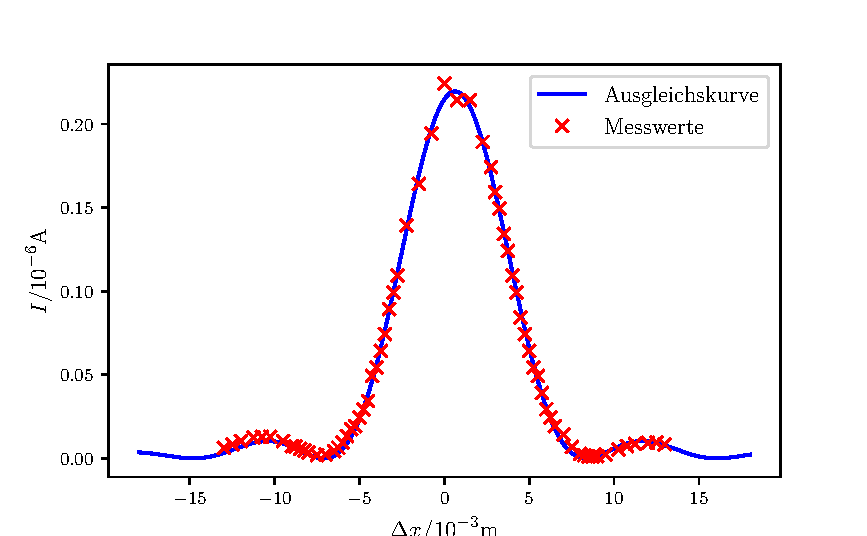
\includegraphics[width=\linewidth-70pt,height=\textheight-70pt,keepaspectratio]{Einzelspalt.pdf}
	\caption{Interferenzmuster der Stromintensitäten eines Einzelspalts in Abhängigkeit von der Verschiebung des Detektors}
	\label{fig:Einzel}
	\end{figure}

\begin{table}[H]
    \centering
    \caption{Die Messdaten am Einfachspalt}
    \label{tab:1}
	\begin{tabular}{| c | c |c||c|c|c| }
		\toprule
		{$\Delta x/10^{-3}\si{\metre}$} & {$I_{\text{mess}}/10^{-7}\si{\ampere}$} & {$I_{\text{eff}}/10^{-7}\si{\ampere}$} &{$\Delta x/10^{-3}\si{\metre}$} & {$I_{\text{mess}}/10^{-7}\si{\ampere}$} & {$I_{\text{eff}}/10^{-7}\si{\ampere}$} \\
		\midrule
		-13,00	&0,070	&0,067	&0,75	&2,150	&2,147\\
		-12,50	&0,090	&0,087	&1,50	&2,150	&2,147\\
		-12,00	&0,110	&0,107	&2,25	&1,900	&1,897\\
		-11,25	&0,130	&0,127	&2,75	&1,750	&1,747\\
		-10,75	&0,135	&0,132	&3,00	&1,600	&1,597\\
		-10,25	&0,135	&0,132	&3,25	&1,500	&1,497\\
		-9,50 	&0,110	&0,107	&3,50	&1,350	&1,347\\
		-9,00 	&0,080	&0,077	&3,75	&1,250	&1,247\\
		-8,75 	&0,078	&0,075	&4,00	&1,100	&1,097\\
		-8,50 	&0,065	&0,062	&4,25	&1,000	&0,997\\
		-8,25 	&0,053	&0,050	&4,50	&0,850	&0,847\\
		-8,00 	&0,040	&0,037	&4,75	&0,750	&0,747\\
		-7,50 	&0,026	&0,023	&5,00	&0,650	&0,647\\
		-7,00 	&0,028	&0,025	&5,25	&0,550	&0,547\\
		-6,50 	&0,050	&0,047	&5,50	&0,500	&0,497\\
		-6,25 	&0,070	&0,067	&5,75	&0,400	&0,397\\
		-6,00 	&0,100	&0,097	&6,00	&0,300	&0,297\\
		-5,75 	&0,140	&0,137	&6,25	&0,250	&0,247\\
		-5,50 	&0,180	&0,177	&6,50	&0,200	&0,197\\
		-5,25 	&0,200	&0,197	&7,00	&0,150	&0,147\\
		-5,00 	&0,250	&0,247	&7,50	&0,075	&0,072\\
		-4,75 	&0,300	&0,297	&8,00	&0,035	&0,032\\
		-4,50 	&0,350	&0,347	&8,25	&0,026	&0,023\\
		-4,25 	&0,500	&0,497	&8,50	&0,019	&0,016\\
		-4,00 	&0,550	&0,547	&8,75	&0,018	&0,015\\
		-3,75 	&0,650	&0,647	&9,00	&0,019	&0,016\\
		-3,50 	&0,750	&0,747	&9,50	&0,032	&0,029\\
		-3,25 	&0,900	&0,897	&10,25	&0,060	&0,057\\
		-3,00 	&1,000	&0,997	&10,75	&0,080	&0,077\\
		-2,75 	&1,100	&1,097	&11,25	&0,094	&0,091\\
		-2,25 	&1,400	&1,397	&12,00	&0,100	&0,097\\
		-1,50 	&1,650	&1,647	&12,50	&0,100	&0,097\\
		-0,75 	&1,950	&1,947	&13,00	&0,090	&0,087\\
		 0,00  &	2,250&	2,247& &&\\			


		\bottomrule
	\end{tabular}
  \end{table}
  \noindent



\subsection{Beugung am Doppelspalt}
Die Messwerte zur Bestimmung der Spaltbreite $b$ und des Spaltabstands $s$ des Doppelspalts sind in der Tabelle \ref{tab:2}  zu finden.
Mit einer Regression der Form 
\[
\begin{split}
I(\Delta x)=4&\cdot A\cdot \left(
\dfrac{\lambda}{\pi\cdot b\cdot\sin{\left(\dfrac{\Delta x-x_0}{L}\right)}}\right)^2\cdot\cos^2{\left(\dfrac{\pi\cdot s\cdot \sin{\left(\dfrac{\Delta x-x_0}{L}\right)}}{\lambda}\right)}\\
&\cdot\sin^2{\left(\dfrac{\pi\cdot b\cdot\sin{\left(\dfrac{\Delta x-x_0}{L}\right)}}{\lambda}\right)}
\end{split}
\]
ergibt sich für den Doppelspalt mit den Startwerten
\begin{equation*}
p_0=
\begin{cases}
\SI{e-4}{\metre}		& \text{für } x_0\\
\SI{e-7}{\ampere}		& \text{für } A_0\\
\SI{e-4}{\metre}		& \text{für } b\\
\SI{e-4}{\metre}		& \text{für } s\\
\end{cases}
\end{equation*}
für die Parameter
\begin{align*}
x_{0} &= \SI{2,69(5)e-4}{\metre}\\
A_0 &= \SI{8,12(8)e-7}{\ampere}\\
b	  &= \SI{1,57(1)e-4}{\metre}\\
s	  &= \SI{2,48(1)e-4}{\metre}\\
\end{align*}


Der zugehörige Graph ist in Abbildung \ref{fig:Doppel} zu sehen.
\begin{table}[H]
    \centering
    \caption{Die Messdaten am Doppelspalt}
    \label{tab:2}
	\begin{tabular}{| c | c |c||c|c|c| }
		\toprule
		{$\Delta x/10^{-3}\si{\metre}$} & {$I_{\text{mess}}/10^{-6}\si{\ampere}$} & {$I_{\text{eff}}/10^{-6}\si{\ampere}$} & {$\Delta x/10^{-3}\si{\metre}$} & {$I_{\text{mess}}/10^{-6}\si{\ampere}$} & {$I_{\text{eff}}/10^{-6}\si{\ampere}$}\\
		\midrule
		
-5,00	&0,1600	&0,1597	&0,25	&3,2000	&3,1997\\
-4,60	&0,1250	&0,1247	&0,50	&2,9000	&2,8997\\
-4,40	&0,0900	&0,0897	&0,60	&2,6000	&2,5997\\
-4,20	&0,0570	&0,0567	&0,80	&2,0000	&1,9997\\
-4,00	&0,0320	&0,0317	&1,00	&1,2000	&1,1997\\
-3,80	&0,0200	&0,0197	&1,20	&0,6000	&0,5997\\
-3,60	&0,0160	&0,0157	&1,40	&0,2200	&0,2197\\
-3,40	&0,0195	&0,0192	&1,60	&0,1200	&0,1197\\
-3,20	&0,0300	&0,0297	&1,80	&0,2600	&0,2597\\
-3,00	&0,0800	&0,0797	&2,00	&0,5200	&0,5197\\
-2,90	&0,1100	&0,1097	&2,20	&0,7800	&0,7797\\
-2,80	&0,1800	&0,1797	&2,40	&0,8000	&0,7997\\
-2,60	&0,3500	&0,3497	&2,60	&0,8000	&0,7997\\
-2,40	&0,5800	&0,5797	&2,80	&0,7000	&0,6997\\
-2,20	&0,7800	&0,7797	&2,90	&0,6000	&0,5997\\
-2,00	&0,9000	&0,8997	&3,00	&0,5000	&0,4997\\
-1,80	&0,8900	&0,8897	&3,20	&0,2500	&0,2497\\
-1,60	&0,7100	&0,7097	&3,40	&0,1750	&0,1747\\
-1,40	&0,4600	&0,4597	&3,60	&0,0750	&0,0747\\
-1,20	&0,2500	&0,2497	&3,80	&0,0250	&0,0247\\
-1,00	&0,1500	&0,1497	&4,00	&0,0180	&0,0177\\
-0,80	&0,2500	&0,2497	&4,20	&0,0150	&0,0147\\
-0,60	&0,7500	&0,7497	&4,40	&0,0220	&0,0217\\
-0,50	&1,0000	&0,9997	&4,60	&0,0340	&0,0337\\
-0,25	&2,0000	&1,9997	&5,00	&0,0740	&0,0737\\
 0,00	&2,9000	&2,8997	&5,50	&0,1000	&0,0997\\

		\bottomrule
	\end{tabular}

	  \end{table}
	  \noindent




\begin{figure}
\centering
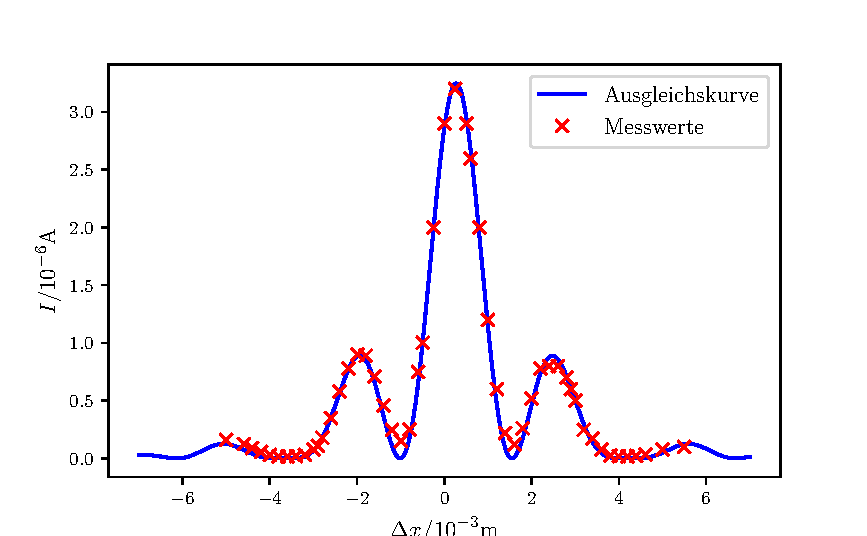
\includegraphics[width=\linewidth-70pt,height=\textheight-70pt,keepaspectratio]{Doppelspalt1.pdf}
\caption{Interferenzmuster der Stromintensitäten des Doppelspalts in Abhängigkeit von der Verschiebung des Detektors}
\label{fig:Doppel}
\end{figure}

